\section{Sensor de Distancia - Implementación con HC-SR04}

En esta sección del artículo se propone el diseño de un circuito que
interaccione con el sensor de distancia HC-SR04, de manera que
sea capaz de activar su funcionamiento y a su vez manipular los datos
que el sensor provee a partir de sus mediciones. 

\subsection{Funcionamiento del HC SR04}

El sensor HC SR04 presenta cuatro pines, de los cuales dos de ellos
son para la alimentación y la conexión a tierra, mientras que los
dos restantes representan la entrada y la salida del sensor. La entrada
(pin de \textit{trigger}) permite disparar una medición del sensor, para
lo cual debe enviarse a este pin un pulso (señal de tensión) de un
mínimo de $10\mu s$ de duración. Por otro lado, luego de dispararse
y realizarse la medición, la salida (pin de \textit{echo}) devuelve un
pulso de duración proporcional a la medición del sensor.

En cuanto a la medición de distancia del sensor, esta se basa en la
emisión de una señal ultrasónica (al activar el pin de \textit{trigger})
que tiene la capacidad de 'rebotar' al encontrar un objeto en
su camino y así poder generar una señal de retorno que es recibida
nuevamente por el sensor. Luego, este calcula el tiempo que tardó
en retornar la señal ultrasónica emitida y devuelve el resultado
provocando un pulso de echo de la misma duración que el tiempo calculado
anteriormente.

Entonces, lo que mide el sensor en realidad es tiempo que puede ser
utilizado para calcular una distancia dado que la velocidad de propagación
de la señal ultrasónica emitida por el sensor es de aproximadamente
$343\frac{m}{s}$ (velocidad del sonido).

Por último, una especificación importante es que el sensor es capaz
de realizar mediciones para objetos que se encuentran a una distancia
de entre 3 y 450 centímetros del mismo, en un ángulo de visión de
15 grados.

\subsection{Diseño del Circuito de Implementación}

A continuación se presenta el pin out del circuito a diseñar:

\begin{figure}[H]
\centering
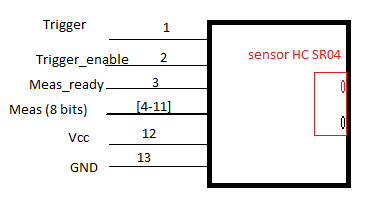
\includegraphics[scale=0.6]{pinOutGenerico.PNG}
\caption{Pin Out - Top Layer}
\end{figure}

Como se ve en la imagen anterior el diseño debe tener en cuenta un
pin de trigger como entrada para activar una medición, el cual a su
vez es habilitado o deshabilitado por un pin de \textit{enable}. Además,
se debe contar con una salida de 8 bits que represente en binario
el tiempo calculado por el sensor HC SR04 en unidades de microsegundos.
Por último, se debe implementar un pin de salida (\textit{meas\_ready})
que indique si la última medición disparada logró su finalización. \newline

Para el diseño se procuró identificar las distintas etapas necesarias
para la resolución del problema planteado para luego avocarse a realizar
circuitalmente cada una de ellas. Luego de analizar los requerimientos
del circuito se propusieron los siguientes módulos: habilitación del
disparo, activación del disparo, procesamiento del echo, generación
de clock, set/reset de (\textit{meas\_ready}). El diagrama en bloques del
proyecto a realizar se puede representar con la siguiente imagen:

\begin{figure}[H]
\centering
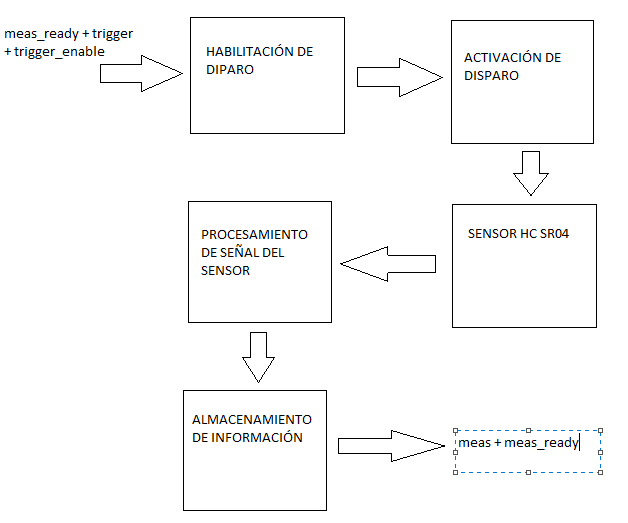
\includegraphics[scale=0.5]{diagramaDeBloquesGenerico.PNG}
\caption{Diagrama en Bloques del Proyecto}
\end{figure}

Además, del diagrama de bloques se pueden identificar dos etapas particulares
las cuales son: módulos anteriores al sensor y módulos posteriores
al sensor. 

A continuación se desarrollará sobre cada módulo en particular, y
dado que lo único que no se diseñará en este proyecto es el sensor
HC SR04, se comenzará analizando los módulos más 'cercanos' al
sensor y particularmente con la etapa \textit{post-sensor}, siguiendo
luego con la etapa \textit{pre-sensor}.

\subsection{Etapa Post-Sensor}

La etapa \textit{post-sensor} cuenta con los módulos de ''procesamiento
de la señal del sensor'' y de ''almacenamiento de los datos procesados'',
los cuales se analizarán a continuación.

\subsubsection{Procesamiento del Echo}

Luego de que el sensor haya realizado la medición, el circuito cuenta
con la señal de \textit{echo} del mismo que es la que debe analizar.
El módulo de procesamiento del \textit{echo} es el encargado de convertir
el pulso de duración variable, otorgado por el sensor HC SR04, a un
número binario de 8 bits. Para esta conversión se utilizará un contador
de al menos 8 bits cuya entrada se conectará al pin de \textit{echo}
del sensor. Suponiendo además que el contador reaccionará ante los
flancos ascendentes de un clock de frecuencia adecuada, se podrá lograr
en el contador la cantidad de veces que cabe un ciclo de clock en
el ancho del pulso de \textit{echo}. Luego, para que el número de 8 bits
represente el tiempo calculado por el sensor en unidades de 100 microsegundos
se puede utilizar el contador con un clock de $10KHz$ (período $T=\frac{1}{10000}s=100\mu s$).

Para abordar el caso de que la señal de echo tenga una duración mayor
a la máxima que se puede representar con 8 bits se podría implementar
un bit extra que indique este problema con el rango de representación.
Es decir, si el bit extra se encuentra encendido significa que la
medición se fue de rango y carece de sentido. Este bit se puede denominar
como ''bit de out of range''.

Por último, para este módulo se debe tener en cuenta que el contador
debe comenzar la cuenta desde cero para cada medición. Para lograr
esto, se puede conectar el pin de reset del contador de 8 bits al
pin de trigger del HC SR04, ya que esto produciría que para el comienzo
de cada medición se imponga un \textit{reset} del contador.\newline

A continuación se presenta el esquemático del diseño del módulo con
componentes discretos:

\begin{figure}[H]
\centering
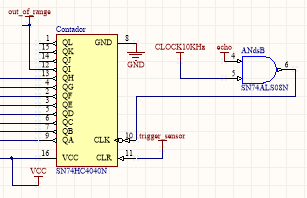
\includegraphics[scale=0.7]{esquemaProcesamientoDeEcho.PNG}
\caption{Esquema del Módulo ''Procesamiento del Echo''}
\end{figure}

Notar que el contador que se muestra en la figura es de 12 bits, lo
cual cumple con los requerimientos de diseño.

En cuanto al clock, su implementación se analizará en el apartado
de ''módulos extras''.

Por otro lado, el echo también define si se está realizando o no una
medición, por ende el módulo debe tener como salida el pin de (\textit{meas\_ready}).
El estado de este pin será definido únicamente por el estado del echo
y por el estado del pin de \textit{out of range}.

\subsubsection{Almacenamiento de la información Procesada}

Una vez procesada la información, es útil guardar esta antes que se
pierda debido a que el módulo que la procesó comience a realizar otras
tareas y la descarte. Para esto se puede utilizar un registro de 8
bits que almacene el tiempo de viaje de la señal del sensor en unidades
de micro-segundos otorgado por el módulo de procesamiento del echo.
Esto es de suma utilidad teniendo en cuenta que el módulo de procesamiento
de echo descarta la información procesada cada vez que se activa una
nueva medición. Por ende, con el módulo de almacenamiento 
se logra obtener información de una medición anterior mientras se
está realizando una nueva. Luego, la salida de este módulo
sería la salida de 8 bits indicada en el pinout del proyecto general.\newline

Sin embargo, para poder implementar esto de manera simple, se requiere
de un registro de 8 bits que se pueda tanto escribir como leer de
manera paralela, y al consultar la existencia de este componente en
el pañol (el pañol es el proveedor de elementos del proyecto) no se
tuvo éxito. Esto genera la necesidad de buscar otras soluciones, lo
cual complejiza el problema. 

Por esto último, se decidió directamente vincular la salida de 8 bits
del circuito con los 8 bits otorgados por el módulo de procesamiento
de echo, lo cual implica una solución simple pero con el costo de
no poder almacenar la medición anterior mientras se está realizando
una nueva.

\subsection{Etapa Pre-Sensor}

La etapa ''pre-sensor'' debe ser capaz de activar el sensor correctamente,
por ende se comenzarán desarrollando los módulos más cercanos al sensor
(dado que es el sensor el que impone los requerimientos).

Los módulos de esta etapa son: ''activación de disparo'' y ''habilitación
de disparo''.

\subsubsection{Activación de Disparo}

Para activar el disparo del sensor es necesario (por la especificación
del mismo) enviar un pulso de duración mayor a $10us$. Por ende el
módulo de activación de disparo debe imponer un pulso con estas características
a su salida en caso de que se indique la activación del disparo medición.
Esta indicación sobre la activación del disparo conformaría la entrada
del módulo y tan solo basta con que sea un bit que represente un 1
lógico en caso de activar un disparo o un 0 en caso de no pretender
una medición.\newline

Hasta aquí se han indicado la entrada y la salida del módulo, pero
debe aclararse también que la medición debe activarse (generación
del pulso mayor a $10us$) una sola vez cuando la entrada este encendida
(1 lógico). Es decir que el módulo debe ser capaz de evitar
el efecto llamado ''retriggering''. Para esto, el módulo solo debe
activar la medición ante el flanco ascendente de la entrada.

Dicho esto, para generar la salida especificada se utilizará el circuito
integrada ''LM555'' en configuración monoestable que genere un pulso
5 veces mayor (en términos de duración) que el mínimo especificado,
es decir, de $50us$. Esta configuración será abordada en el apartado
de ''módulos extras'', pero es importante tener en cuenta que para
lograr que la configuración funcione correctamente es necesario ingresar
a este con un pulso de menor a $50us$ y además debe ser ''invertido'',
es decir que el estado que debe ser menor a $50us$ es el 0
lógico.\newline

Luego, se decidió implementar un circuito conformado por una resistencia
y un capacitor que ante la entrada genere una señal análogica la cual
mediante una compuerta de tipo ''schmitt trigger'' se pueda traducir
en un pulso de ancho configurable por el valor de la resistencia y
el capacitor. A continuación se presenta un esquema del circuito mencionado:

\begin{figure}[H]
\begin{centering}
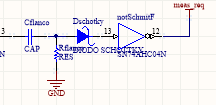
\includegraphics[scale=1]{generadorDePulsoMenor50us.PNG}
\par\end{centering}
\caption{Esquema - Generador de Pulso Menor a $50us$}
\end{figure}

Se puede notar que en la implementación entra en juego un diodo, el
cual es muy importante ya que la señal provocada por la resistencia
genera un pulso de tensión positiva ante un flanco ascendente de la
entrada, pero también genera un pulso de tensión negativa ante el
flanco descendente de la misma y es para filtrar este último pulso
que existe el diodo en el esquema. En particular, el diodo debe ser
de tipo ''schotcky'' para no producir caidas de tensión elevadas.

Por último, cabe mencionar que el pulso generado por la configuración
presentada en la figura también se podría ajustar para ingresarlo
directamente al pin de trigger del sensor HC SR04, pero de todas maneras
se decidió la implementación de la configuración monoestable del LM555
para mayor precisión en el ancho del pulso enviado al sensor.

\subsubsection{Habilitación de Disparo}

Este módulo tiene como objetivo habilitar el disparo de la medición.
Para que esto suceda es necesario que los pines de \textit{trigger\_enable}
y \textit{trigger} se encuentren encendidos pero además debe asegurarse
que no exista ninguna medición en proceso.\newline

Dadas estas especificaciones del módulo se planteó el siguiente circuito:

\begin{figure}[H]
\begin{centering}
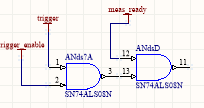
\includegraphics[scale=1]{habilitacionDeDisparo.PNG}
\caption{Diseño Circuital - Habilitación de Disparo}
\par\end{centering}
\end{figure}

\subsection{Módulos Extras}

A continuación se abordará el diseño de los módulos de ''clock''
(utilizado en el procesamiento del echo) y de ''LM555 monoestable''
(utilizado en la activación de disparo).

\subsubsection{LM555 Monoestable}

Una vez habilitado el disparo debe activarse el mismo enviando un
pulso de un ancho mínimo de $10\mu s$ al pin de \textit{trigger} del
HC SR04. Para esto se decidió usar un multivibrador monoestable, logrado
mediante el integrado LM555. El pin out del circuito integrado
es el siguiente:

\begin{figure}[H]
\centering
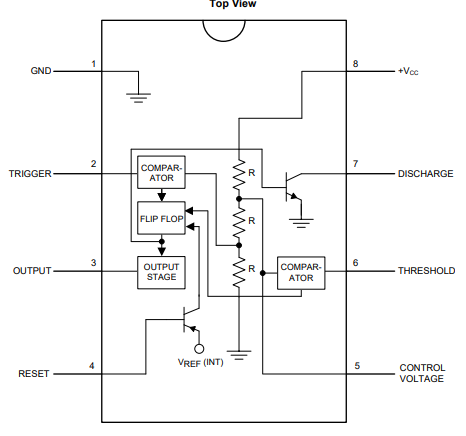
\includegraphics[scale=0.5]{pinOutLM55(a).PNG}
\qquad
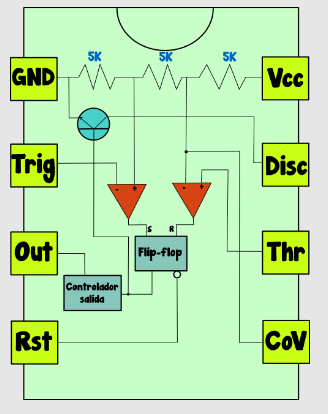
\includegraphics[scale=0.5]{pinOutLM55(b).PNG}
\caption{Pin Out - LM555}
\end{figure}

Vale aclarar, que los amplificadores operacionales representados en
la imagen de la derecha simulan la función de comparación.

Para utilizar el LM555 (el nombre '555' es debido al divisor resistivo
de 3 resistencias de $5K\Omega$ ) en configuración monoestable se
procederá a realizar el siguiente circuito:

\begin{figure}[H]
\centering
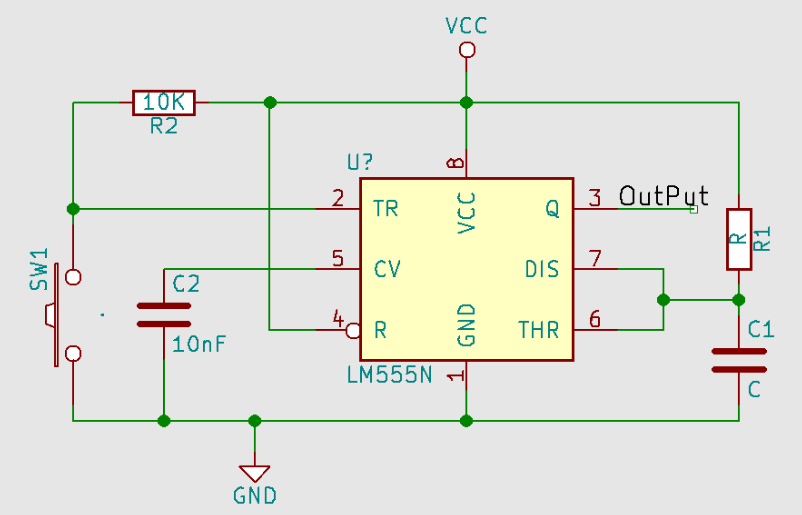
\includegraphics[scale=0.4]{monoestable555.PNG}
\caption{Configuración Monoestable - LM555}
\end{figure}

Como se puede deducir a partir de las imágenes anteriores, al excitar
el pin de trigger con una tensión mayor a $\frac{1}{3}$ de Vcc,
se activará la salida a la vez que se permitirá la carga del capacitor
$C1$. Luego, al llegar el capacitor a una tensión mayor a $\frac{2}{3}$
de Vcc se reseteará la salida debido a la comparación del pin de threshold,
y el capacitor se descargará nuevamente mediante la conexión a tierra.
Esto produce que la salida se encienda tan solo durante el lapso de
tiempo que el capacitor tarda en cargarse hasta $\frac{2}{3}$ de
Vcc. Por ende, la duración del pulso se puede calcular de la siguiente
manera:

\begin{equation}
V_{capacitor}=V_{cc}(1-e^{\frac{-t}{R_{1}C_{1}}})
\end{equation}

Luego, 
\vspace{5mm}
\begin{equation}
V_{capacitor}=\frac{2}{3}V_{cc}\Longleftrightarrow e^{\frac{-t}{R_{1}C_{1}}}=\frac{1}{3}\Longleftrightarrow t=ln(3)R_{1}C_{1}    
\end{equation}

\vspace{5mm}
Dicho esto, para lograr un pulso de $50\mu s$ (esta duración de pulso
es adecuada ya que es 5 veces mayor al ancho mínimo del pulso requerido
por el sensor HC SR04) se puede utilizar una resistencia de $5K\Omega$
y un capacitor de $10nF$.

\subsubsection{Generación de Clock}

Como se ha visto, para el módulo de procesamiento del echo es necesario
un clock de $10KHz$. La implementación de un clock puede realizarse
de varias maneras, de las cuales una es hacer uso nuevamente del LM555
en configuración astable como se muestra a continuación:

\begin{figure}[H]
\begin{centering}
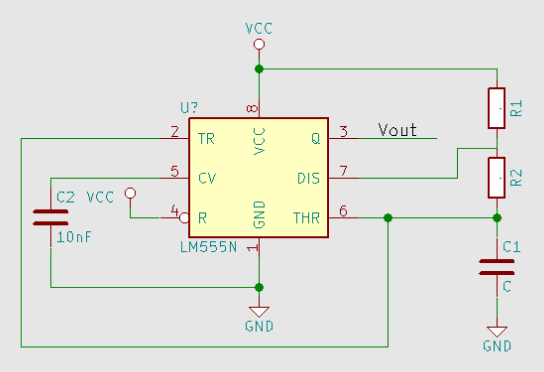
\includegraphics[scale=0.4]{astable555.PNG}
\par\end{centering}
\caption{Configuración Astable - LM555}
\end{figure}

En esta configuración el capacitor $C1$ comenzará descargado provocando
que inicialmente la salida sea nula, sin embargo comenzará a cargarse
de forma que la tensión entre placas puede modelarse mediante la siguiente
expresión: 
\begin{equation}
    V_{C1}=V_{cc}(1-e^{-\frac{t}{(R_{1}+R_{2})C_{1}}})   
\end{equation}


Luego, cuando la tensión del capacitor supere $\frac{1}{3}$ de $V_{cc}$
la salida se activará (será un 1 lógico) hasta que la tensión entre
placas del capacitor que se sigue cargando supere $\frac{2}{3}$ de$V_{cc}$.
Una vez que se superan los dos tercios de $V_{cc}$ la salida vuelve
a anularse (cero lógico) y el capacitor comienza a descargarse comportandose
según lo describe la siguiente igualdad:

\begin{equation}
V_{C1}=V_{cc}e^{-\frac{t}{R_{2}C_{1}}}
\end{equation}

La descarga se producirá hasta que la tensión vuelva a ser $\frac{1}{3}$
de $V_{cc}$ y logre activar nuevamente la salida. Este proceso se
repetirá sucesivamente hasta que se desconecte la alimentación $V_{cc}$,
por ende, se logra obtener una señal cuadrada periódica que simule
un clock. Además, esta señal se mantiene representando un 1
lógico durante el tiempo para el cual la tensión en el capacitor $C1$
se mantiene cargandosé entre $\frac{1}{3}$ y $\frac{2}{3}$ de $V_{cc}$,
y representa, en cambio, un 0 lógico cuando se mantiene descargándose
entre $\frac{2}{3}$ y $\frac{1}{3}$ de $V_{cc}$. A continuación
se presenta el cálculo del tiempo de encendido de la señal (1
lógico) y del tiempo de apagado de la misma (0 lógico).\\
\vspace{5mm}
Durante la carga:
\begin{equation}
V_{C1}=\frac{1}{3}V_{cc}\Longleftrightarrow t=ln(\frac{3}{2})(R_{1}+R_{2})C_{1}    
\end{equation}
\begin{equation}
V_{C1}=\frac{2}{3}V_{cc}\Longleftrightarrow t=ln(3)(R_{1}+R_{2})C_{1}
\end{equation}
\begin{equation}
\Rightarrow t_{ON}=[ln(3)-ln(\frac{3}{2})][(R_{1}+R_{2})C_{1}]=ln(2)[(R_{1}+R_{2})C_{1}]
\end{equation}
\vspace{5mm}
Durante la descarga:
\begin{equation}
V_{C1}=\frac{1}{3}V_{cc}\Longleftrightarrow t=ln(3)R_{2}C_{1}
\end{equation}
\begin{equation}
V_{C1}=\frac{2}{3}V_{cc}\Longleftrightarrow t=ln(\frac{3}{2})R_{2}C_{1}
\end{equation}
\begin{equation}
\Rightarrow t_{OFF}=[ln(3)-ln(\frac{3}{2})]R_{2}C_{1}=ln(2)R_{2}C_{1}
\end{equation}

\vspace{5mm}
Dadas estos resultados análiticos, y considerando que en un clock
se debe cumplir que $t_{ON}=t_{OFF}$, entonces se debe elegir una
resistencia $R_{2}$ mucho mayor que $R_{1}$ de manera que
$R_{1}+R_{2}\simeq R_{2}$.

Además, a partir de lo calculado se obtiene que $f_{clock}=\frac{1}{t_{ON}+t_{OFF}}\simeq\frac{1}{2ln(2)R_{2}C_{2}}=\frac{1}{ln(4)R_{2}C_{2}}$.
Luego, para un clock de $10KHz$ se obtiene la siguiente relación
entre los valores de los componentes:

\[
    R_{2}\gg R_{1},\\
    R_{2}C_{2}\simeq7.2x10^{-5}
\]

\vspace{5mm}
Luego, esto se puede lograr con $R_{1}=1K\varOmega$, $R_{2}=72K\varOmega$
y $C_{1}=1nF$.

\subsection{Aspectos a Mejorar}

Hasta aquí el diseño del circuito cumple con los requerimientos que
motivaron su realización. Sin embargo existen algunos aspectos en
este que se pueden identificar como mejorables.

Uno de ellos es el almacenamiento de la información, es decir, el
hecho de que no se guarda en un registro auxiliar el resultado de
procesamiento de las mediciones del sensor es un hecho que se puede
revertir a pesar de no contar con un registro de 8 bits de lectura
y escritura en paralelo. Para atacar este problema se podría pensar
en un mecanismo que permita la implementación de registros con lectura
y/o escritura en seria, pero también se pueden utilizar dos registros
de 4 bits con su lectura y escritura en modo paralelo, dado que los
registros de 4 bits con estas características son más accesibles que
los de 8 bits en cuanto a su stock.

Por otro lado, para procesar la medición del sensor se utiliza un
contador de 12 bits, de los cuales solo se utilizan 9 (ocho para contar
y uno para indicar fuera de rango). Esto implica que existen tres
bits que se estan desaprovechando. Para su mejor provecho se podría
aumentar la frecuencia del clock que ingresa al contador provocando
así que las unidades de medida del contador sean menores a $100us$,
lo cual daría mayor precisión a la medición. Si esto se implementa,
también sería necesario un \textit{shift register} para luego obtener
nuevamente la salida de 8 bits en unidades de $100us$ que se requiere.

\subsection{Conclusión}

Como conclusión luego de abordar el diseño del proyecto a partir de
los requerimientos especificados en primera instancia, que luego dió
lugar a múltiples variables a tener en cuenta, se puede decir fue
crucial atacar la problemática de cada una de ellas por separado.
De esta manera, los \textit{requerimientos padres} (los requerimientos
principales fueron los pines de entrada y de salida del circuito,
y lo que cada uno de ellos debía representar) dieron origen a \textit{requerimientos
hijos} los cuales a su vez también podían desprender otros nuevos
requerimientos, pero se pudo afrontar cada uno de ellos por separado
conformando bloques sólidos que tenían como característica su capacidad
de ser testeado o probado de una manera simple.

Por otro lado, el diseño también fue un desafío ya que antes de tomar
una decisión o definir una idea surgieron muchas variantes para una
misma solución y por ende se debió analizar cual de todas ellas presentaba
mejor relación entre costo y beneficio, siendo el costo definido principalmente
por el tiempo necesario de inversión en el diseño. 